% Considerações finais
\chapter{Conclusão} \label{ch:conclusao}

Este capítulo apresenta na seção \ref{sec:cronograma-atividades} o cronograma das atividades que guiarão a continuidade do trabalho durante o próximo semestre. Na seção \ref{sec:limitacoes} são mostradas algumas limitações já conhecidas deste trabalho.

\section{Cronograma de Atividades} \label{sec:cronograma-atividades}

A figura \ref{fig:cronograma-atividades} adiante apresenta o cronograma de atividades a ser seguido durante o próximo semestre. Vale salientar que todas as datas apresentadas na figura são estimativas, portanto, são datas aproximadas. Dessa forma, podem ocorrer variações nas datas planejadas.

\begin{figure}[!htb]
   \centering
   \frame{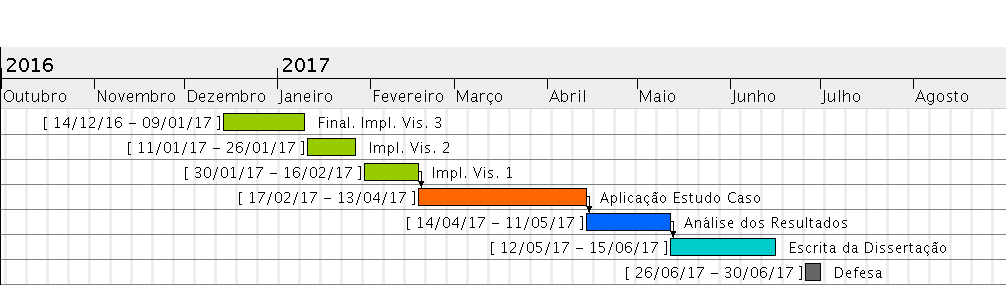
\includegraphics[scale=0.45]{Imagens/cronograma.png}}
   \textsf{\caption[Cronograma de atividades.]{Cronograma de atividades.\label{fig:cronograma-atividades}}}
\end{figure}

Após a qualificação, será dada continuidade a implementação da visualização 3, o grafo de chamadas. Será implementada a opção de o desenvolvedor ou arquiteto usuário do sistema obter acesso ao código-fonte responsável por desvios de desempenho indicados na visualização. Esta atividade durará até a primeira metade do mês de janeiro/17.

Após a conclusão da implementação da visualização do grafo de chamadas, será implementada a visualização 2 - sumarização dos cenários. Essa atividade foi escolhida por ser menos complexa do que a visualização 1, evolução do desempenho, e a previsão de duração é até o final do mês de janeiro/17. Na sequência, para finalizar a etapa de desenvolvimento do trabalho, a visualização de evolução do desempenho será implementada, em tarefa que tem conclusão prevista para a primeira metade de fevereiro/17.

Passada a etapa de desenvolvimento, serão iniciados os estudos empíricos planejados, conforme descritos neste documento. Essa etapa, por envolver desenvolvedores e arquitetos dos sistemas escolhidos, terá maior tempo de duração e está prevista para ser finalizada na primeira quinzena de abril/17. Terá duração total de aproximadamente 50 dias.

Em abril/17, está planejado que se inicie as análises dos estudos de caso realizados, em tarefa que durará, aproximadamente, 25 dias. Pretende-se analisar qualitativamente os dados obtidos para, então, obter os resultados do trabalho.

Após essa etapa, será retomada a escrita do documento, relatando o desenvolvimento das visualizações 1 e 2, os detalhes da aplicação dos estudos de caso, os resultados obtidos nesses estudos, bem como será revisto e, se cabível, refinado cada capítulo do documento. A defesa desta dissertação de mestrado é planejada para a última semana de junho/17.

\section{Limitações} \label{sec:limitacoes}

Algumas limitações do trabalho são conhecidas, em particular para a visualização do grafo de chamadas:
\begin{itemize}
	\item \textit{Tamanho do grafo}: a quantidade de nós com desvios de desempenho de uma versão para outra do software pode ser em grande quantidade de modo a comprometer o desempenho da própria visualização, comprometer a usabilidade e a visibilidade ou, até mesmo, inviabilizá-la. Embora medidas tenham sido tomadas para minimizar esse impacto - como, por exemplo, o agrupamento de nós não relacionados com nós de desvio ou adicionados - há possibilidades de acontecer;
	\item \textit{Evoluções espaçadas ou bruscas}: caso sejam analisadas duas versões muitos distantes entre si, as modificações podem ser enormes, fazendo com que o grafo gerado seja grande e complexo, resultando no problema do tamanho do grafo apresentado no item anterior. Para análises desse tipo, pode ser recorrido a uma análise em alta granularidade. O ideal ao utilizar a ferramenta é analisar versões próximas, para beneficiar-se da baixa granularidade apresentada pelo grafo de chamadas.
\end{itemize}

Também pode ser considerada uma limitação, herdada do \textit{PerfMiner}, o fato de o conjunto de visualizações apresentar apenas dados do atributo de qualidade de  desempenho. No entanto, a ferramenta está apta a atender a outros atributos de qualidade.